\section{Introduction}
\label{sec:introduction}

The successful implementation of task-oriented dialogue (TOD) systems begins with the precise recognition of user intents.
By accurately discerning the queries embedded in user inputs and routing them to the relevant components, the systems can adeptly respond, thereby effectively fulfilling user requests. 
Generally, these systems are constructed on the assumption that each user utterance is exclusively linked to a single intent, which often diverges from practical scenarios.

Contrary to the conventional setting, the task of \textbf{Multi-Intent Detection (MID)} presents a more nuanced and comprehensive challenge for TOD systems, permitting users to express multiple intentions simultaneously.
The problems posed by MID are not only more demanding but also more realistic---for reference, \citet{gangadharaiah-narayanaswamy-2019-joint} reported that over half of the total instances (52\%) from Amazon's in-house dialogue dataset contain multiple intents, underscoring the practical significance of the task.

\begin{figure}
    \begin{center}
        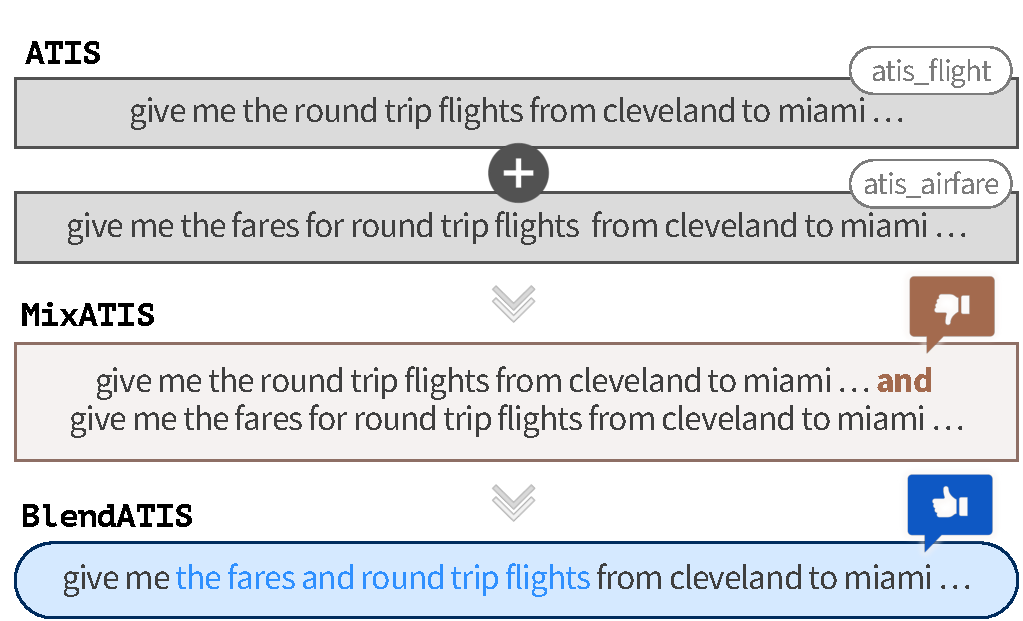
\includegraphics[scale=0.45]{images/Figure_0.pdf} 
        \caption{
        An example that underscores the distinct features of MixX and BlendX.
        In contrast to MixX, which relies on simple concatenations, BlendX steps beyond by simulating more realistic and complex cases often found in real-world conversations.
        }
        \label{fig:comparison_concat}
    \end{center}
\end{figure}

\begin{figure*}[t]
    \begin{center}
        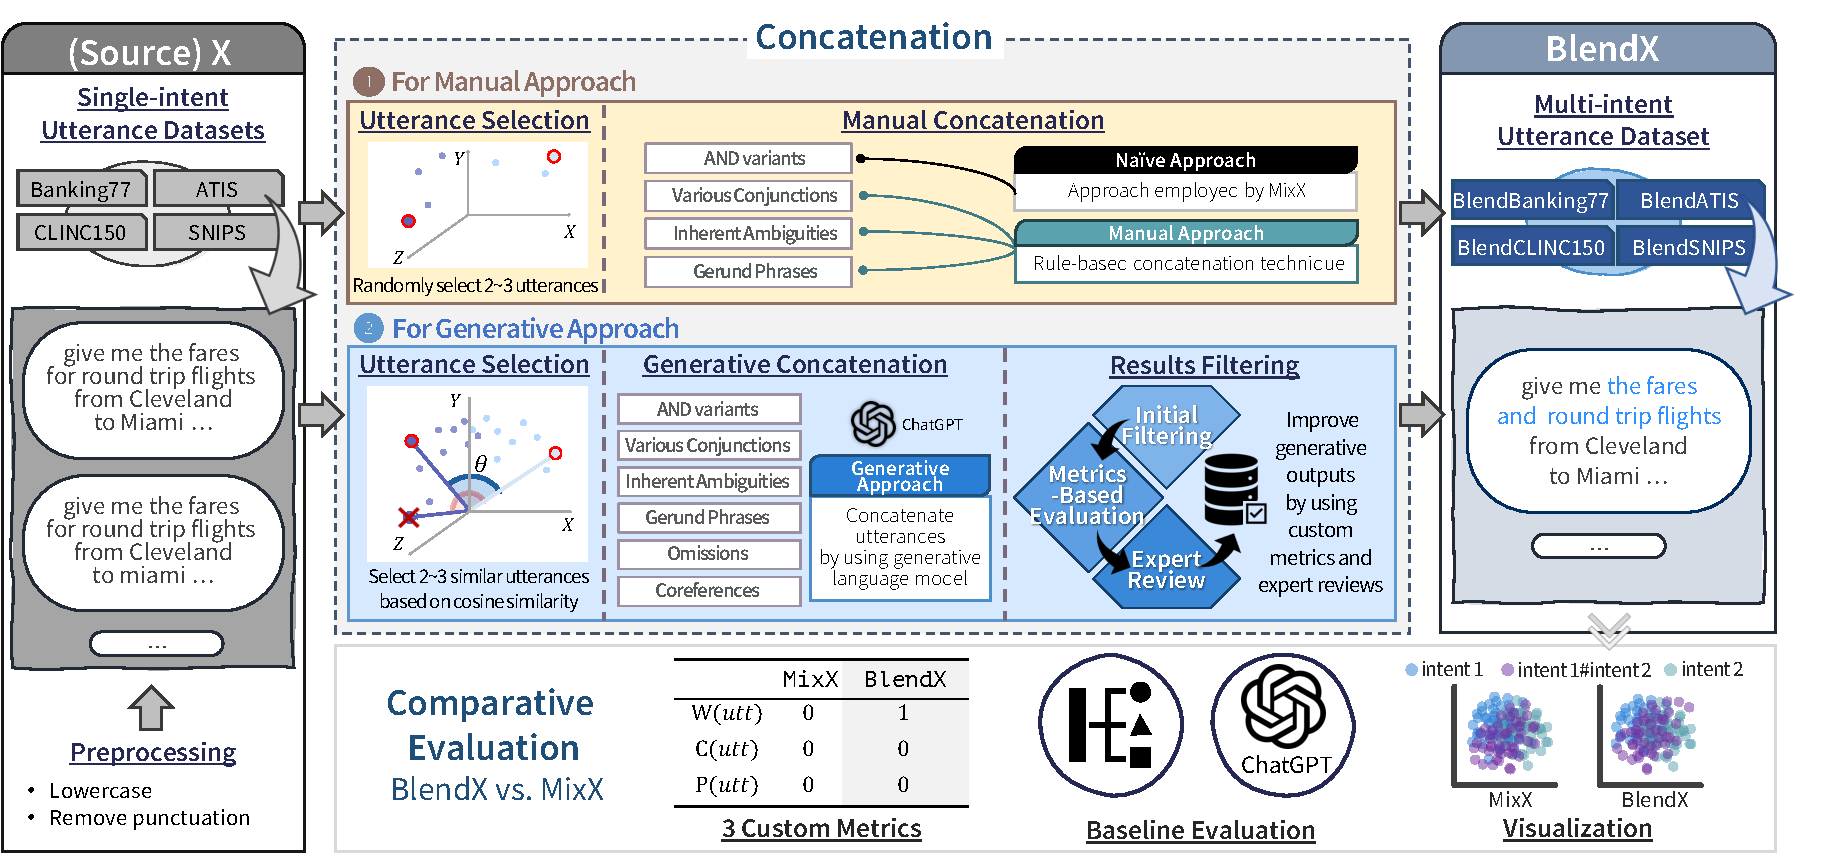
\includegraphics[scale=0.53]{images/Figure_1.pdf} 
        \caption{
        An overview of the BlendX construction framework. 
        Initially, we preprocess four source datasets: ATIS, Banking77, CLINC150, and SNIPS.
        We then select single-intent utterances from these datasets.
        These utterances are combined using both Manual and Generative approaches.
        It is important to note that utterances are kept separate and not mixed across datasets.
        Following the merging process, all resultant datasets are compiled to form BlendX.
        We particularly highlight non-trivial combinations, such as omissions, which are indicated within the blue rounded box on the rightmost side of the framework.
        Finally, BlendX is evaluated using three methods: custom metrics, baseline evaluation, and visualization.
        }
        \label{fig:overall}
    \end{center}
\end{figure*}

Despite the ongoing interest in MID, we find it surprisingly notable that resources supporting this research direction are quite limited.
Most studies on MID rely on two representative datasets, i.e., \textit{MixATIS} and \textit{MixSNIPS} \citeplanguageresource{qin-etal-2020-agif}.
They serve as extensions of the classic single-intent detection datasets---\textit{ATIS} \citeplanguageresource{mansour2021atis} and \textit{SNIPS} \citeplanguageresource{coucke2018snips}---modified to include scenarios that involve multiple intents.

Unfortunately, in spite of its pervasive adoption within the domain, \textbf{MixX}\footnote{A term encompassing both MixATIS and MixSNIPS, as well as the framework used to create the datasets.} \citeplanguageresource{qin-etal-2020-agif} has faced criticism for the simplicity inherent in their construction.
\citet{larson2022survey} highlighted the insufficient diversity in the connectives used to merge multiple utterances into a unified expression in the construction of MixX.
That is, MixX features merely four types of coordinating conjunctions: \texttt{`and'}, \texttt{`and then'}, \texttt{`and also'}, and \texttt{`,(comma)'}, patterns that are susceptible to detection by cutting-edge models.\footnote{For instance, a smart model may exploit the na\"ive patterns to identify the number of intents in an utterance without grasping the utterance's overall semantics.}
Consequently, this casts doubt on the validity of evaluations related to recent MID approaches, especially since the principal components of these evaluations generally lean on the aforementioned datasets, MixX.

In this context, we argue that obvious and urgent needs exist for establishing a more rigorous testbed for MID, as shown in Figure \ref{fig:comparison_concat}.
Remarkably, this comes despite the minimal effort noted in the literature to address the issue.
While recent work on MID largely focuses on devising new methodological schemes---evaluated within fixed, simple environments---we aim to offer orthogonal enhancement to the field by introducing a suite of upgraded datasets, dubbed \textbf{BlendX}.

We explore the limitations present in the current form of MID datasets and propose curated datasets featuring more complex and varied patterns.
Initially, we propose pragmatic rules for manually merging single-intent utterances, utilizing an expanded array of connectors that allow us to diverge from the simple heuristics employed in MixX.

Moreover, we consider the automated concatenation of utterances, facilitated by leveraging OpenAI's ChatGPT\footnote{In particular, we employ \texttt{gpt-3.5-turbo-0613}.}.
We find that, although ChatGPT is versatile, its na\"ive utilization struggles to merge  given utterances while preserving their original intents.
To maximize its efficacy, we introduce a similarity-based strategy for utterance selection, aiding the model to operate in more realistic settings without being excessively challenging.

In addition, we propose three intuitive metrics designed to assess the quality of the constructed datasets.
Our analysis with these metrics demonstrates that BlendX significantly outperforms its predecessors in terms of complexity and diversity.

Lastly, we revisit state-of-the-art MID models, i.e., TFMN \cite{chen-etal-2022-transformer} and SLIM \cite{9747477}, as well as ChatGPT to evaluate their performance on BlendX.
We discover that MID models struggle to adapt to the distinctive patterns present in BlendX, prompting a re-evaluation of the current state in MID literature.
We also provide extensive analysis of BlendX's attributes, shedding light on its unique contributions.